\chapter{AINDA FALANDO DO LINUX}
\label{apb:linux}
\vspace{-2cm}

Neste capítulo será abordado o surgimento e a evolução do sistema operacional Linux.

\section*{\hspace{1.3cm}APÊNDICE B.1 - MELHORIAS PARA O LINUX EM UM AMBIENTE COORPORATIVOS DE DUAS GRNDES FRNTES INTERPRETATIVAS}
\sectionmark{\protect\parbox{.9\textwidth}{APÊNDICE B.1 - MELHORIAS PARA O LINUX EM UM AMBIENTE COORPORATIVOS DE DUAS GRNDES FRNTES INTERPRETATIVAS}}
\label{secapb:linux}
Atualmente, ... 

\begin{itemize}
\item \textbf{Facilidade de acesso aos recursos:} consiste em ser totalmente transparente ao usuário a maneira como funciona um computador, ou seja, para um usuário comum \index{usuário!comum} não importa como um arquivo que está em um disquete será lido, mas sim que o mesmo será lido, resumindo, um usuário \index{usuário} não precisa saber como será realizado essa ação e suas inúmeras etapas. \cite{machado};
\end{itemize}

%%\begin{figure}[htbp]
%\begin{figure}[H]
%\tiny \caption{\small Novo sistema operacional.}
%\vspace{-0.3 cm}
%\begin{center}
%\begin{psfrags}
%\epsfxsize=4cm
%\centerline{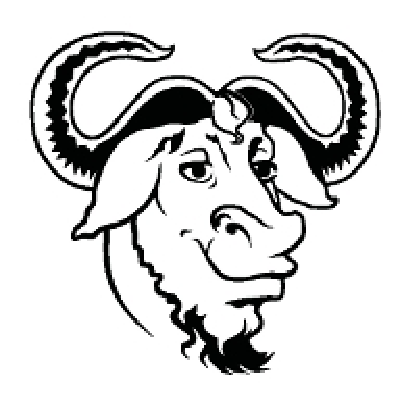
\includegraphics[width=4.0 cm]{./apb/gnu-linux.eps}}
%\end{psfrags}
%{\small Fonte: \citeonline{machado}}
%\end{center}
%\end{figure}

Para facilitar a vida dos usuários, um exemplo de tabela longa.

\begin{centering}
\footnotesize
\begin{longtable}{c|c|c|c|c|c|c|c|c|c|c}
\captionsetup{width=14.8cm}
\caption{\label{tab:5solIEEE}Espaço ~~de ~busca ~combinatório ~reduzido ~($EBCR$) ~de 10, 5, 3 e 2 ~soluções com \textit{gap} de 5\% Para IEEE}\\
\hline
\multirow{3}{*}{Ramos} & \multicolumn{10}{c}{Número Máximo de linhas}\tabularnewline
\cline{2-11} 
 & \multicolumn{2}{c|}{poolreplace=0} & \multicolumn{4}{c|}{poolreplace=1} & \multicolumn{4}{c}{poolreplace=2}\tabularnewline
\cline{2-11} 
 & 5 sol. & 2 sol. & 10 sol. & 5 sol. & 3 sol. & 2 sol. & 10 sol. & 5 sol. & 3 sol. & 2 sol.\tabularnewline
\hline 
\hline
\endfirsthead
\caption[]{(Continuação da tabela da página anterior)}\\
\hline
\multirow{3}{*}{Ramos} & \multicolumn{10}{c}{Número Máximo de linhas}\tabularnewline
\cline{2-11} 
 & \multicolumn{2}{c|}{poolreplace=0} & \multicolumn{4}{c|}{poolreplace=1} & \multicolumn{4}{c}{poolreplace=2}\tabularnewline
\cline{2-11} 
 & 5 sol. & 2 sol. & 10 sol. & 5 sol. & 3 sol. & 2 sol. & 10 sol. & 5 sol. & 3 sol. & 2 sol.\tabularnewline
\hline     
\hline
\endhead
\hline
\multicolumn{11}{r}{\emph{continua.}}
	\endfoot
	\multicolumn{11}{r}{\emph{Fim.}}
	\endlastfoot
\hline 
$n_{1-2}$  & 3 & 1 & 3 & 4 & 2 & 1 & 4 & 3 & 2 & 0\tabularnewline
\hline 
$n_{1-3}$  & 0 & 0 & 0 & 0 & 0 & 0 & 0 & 0 & 0 & 0\tabularnewline
\hline 
$n_{1-5}$  & 1 & 1 & 1 & 1 & 1 & 1 & 1 & 1 & 1 & 1\tabularnewline
\hline 
$n_{2-4}$  & 0 & 0 & 0 & 0 & 0 & 0 & 0 & 0 & 0 & 0\tabularnewline
\hline 
$n_{2-6}$  & 0 & 0 & 0 & 0 & 0 & 0 & 0 & 0 & 0 & 0\tabularnewline
\hline 
$n_{3-9}$  & 0 & 0 & 0 & 0 & 0 & 0 & 0 & 0 & 0 & 0\tabularnewline
\hline 
$n_{3-24}$  & 1 & 1 & 1 & 1 & 1 & 1 & 1 & 1 & 1 & 1\tabularnewline
\hline 
$n_{4-9}$  & 0 & 0 & 0 & 0 & 0 & 0 & 0 & 0 & 0 & 0\tabularnewline
\hline 
$n_{5-10}$  & 0 & 0 & 0 & 0 & 0 & 0 & 0 & 0 & 0 & 0\tabularnewline
\hline 
$n_{6-10}$  & 1 & 1 & 1 & 1 & 1 & 1 & 1 & 1 & 1 & 1\tabularnewline
\hline 
$n_{7-8}$  & 3 & 2 & 3 & 2 & 3 & 3 & 2 & 3 & 2 & 3\tabularnewline
\hline 
$n_{8-9}$  & 0 & 0 & 0 & 0 & 0 & 0 & 0 & 0 & 0 & 0\tabularnewline
\hline 
$n_{8-10}$  & 0 & 0 & 0 & 0 & 0 & 0 & 0 & 0 & 0 & 0\tabularnewline
\hline 
$n_{9-11}$  & 0 & 0 & 0 & 0 & 0 & 0 & 0 & 0 & 0 & 0\tabularnewline
\hline 
$n_{9-12}$  & 0 & 0 & 0 & 0 & 0 & 2 & 0 & 0 & 0 & 0\tabularnewline
\hline 
$n_{10-11}$  & 1 & 0 & 1 & 0 & 1 & 1 & 0 & 1 & 0 & 1\tabularnewline
\hline 
$n_{10-12}$  & 1 & 1 & 1 & 1 & 1 & 1 & 1 & 1 & 1 & 1\tabularnewline
\hline 
$n_{11-13}$  & 1 & 1 & 1 & 1 & 1 & 1 & 1 & 1 & 1 & 1\tabularnewline
\hline 
$n_{11-14}$  & 0 & 0 & 0 & 0 & 0 & 1 & 0 & 0 & 0 & 0\tabularnewline
\hline 
$n_{12-13}$  & 0 & 0 & 0 & 0 & 0 & 0 & 0 & 0 & 0 & 0\tabularnewline
\hline 
$n_{12-23}$  & 0 & 0 & 0 & 0 & 0 & 0 & 0 & 0 & 0 & 0\tabularnewline
\hline 
$n_{13-23}$  & 0 & 0 & 0 & 0 & 0 & 0 & 0 & 0 & 0 & 0\tabularnewline
\hline 
$n_{14-16}$  & 1 & 1 & 1 & 1 & 1 & 1 & 1 & 1 & 1 & 1\tabularnewline
\hline 
$n_{15-16}$  & 0 & 0 & 0 & 0 & 0 & 0 & 0 & 0 & 0 & 0\tabularnewline
\hline 
$n_{15-21}$  & 0 & 0 & 0 & 0 & 0 & 0 & 0 & 0 & 0 & 0\tabularnewline
\hline 
$n_{15-24}$  & 0 & 0 & 0 & 0 & 0 & 0 & 0 & 0 & 0 & 0\tabularnewline
\hline 
$n_{16-17}$  & 0 & 0 & 0 & 0 & 0 & 0 & 0 & 0 & 0 & 0\tabularnewline
\hline 
$n_{16-19}$  & 0 & 0 & 0 & 0 & 0 & 0 & 0 & 0 & 0 & 0\tabularnewline
\hline 
$n_{17-18}$  & 0 & 0 & 0 & 0 & 0 & 0 & 0 & 0 & 0 & 0\tabularnewline
\hline 
$n_{17-22}$  & 0 & 0 & 0 & 0 & 0 & 0 & 0 & 0 & 0 & 0\tabularnewline
\hline 
$n_{18-21}$  & 0 & 0 & 0 & 0 & 0 & 0 & 0 & 0 & 0 & 0\tabularnewline
\hline 
$n_{19-20}$  & 0 & 0 & 0 & 0 & 0 & 0 & 0 & 0 & 0 & 0\tabularnewline
\hline 
$n_{20-23}$  & 1 & 1 & 1 & 1 & 1 & 1 & 1 & 1 & 1 & 1\tabularnewline
\hline 
$n_{21-22}$  & 0 & 0 & 0 & 0 & 0 & 0 & 0 & 0 & 0 & 0\tabularnewline
\hline 
$n_{1-8}$  & 0 & 0 & 0 & 0 & 0 & 0 & 0 & 0 & 0 & 0\tabularnewline
\hline 
$n_{2-8}$  & 0 & 0 & 0 & 0 & 0 & 1 & 0 & 0 & 0 & 0\tabularnewline
\hline 
$n_{6-7}$  & 0 & 0 & 0 & 0 & 0 & 2 & 0 & 0 & 0 & 0\tabularnewline
\hline 
$n_{13-14}$  & 0 & 0 & 0 & 0 & 0 & 1 & 0 & 0 & 0 & 0\tabularnewline
\hline 
$n_{14-23}$  & 1 & 0 & 1 & 0 & 1 & 1 & 0 & 1 & 0 & 1\tabularnewline
\hline 
$n_{16-23}$  & 0 & 0 & 0 & 0 & 0 & 0 & 0 & 0 & 0 & 0\tabularnewline
\hline 
$n_{19-23}$  & 0 & 0 & 0 & 0 & 0 & 0 & 0 & 0 & 0 & 0\tabularnewline
\hline 
\hline 
F.O & 220.28 & 220.28 & 220.28 & 220.28 & 220.28 & 220.28 & 220.28 & 220.28 & 220.2 & 220.2\tabularnewline
\hline
\hline
\multicolumn{11}{l}{\small{Fonte: Dados da pesquisa do autor.}}\tabularnewline
\end{longtable}
\par\end{centering}


